\section{Methods}
\label{sec:methods}    
    In this section the methodologies implemented are illustrated, starting from the
    dataset used, the preprocessing steps and the models implemented.

    \subsection{Dataset}
    \label{subsec:dataset}
        The dataset used in this project is a collection of Trip Advisor reviews, taken
        from kaggle\footnote{\url{https://www.kaggle.com/datasets/andrewmvd/trip-advisor-hotel-reviews}}.
        Such dataset contains 20491 english reviews of hotels, labelled with a score from
        1 to 5 stars (labels 0 to 4). To grant a more balanced benckmark, all the reviews with a
        length greater than 256 tokens according to the RoBERTa tokenizer were 
        dropped, resulting in a final dataset of 18273 reviews. Such choice was
        made to make a compromise between the maximum depth of the LSTM Networks
        in order to avoid vanishing gradients, and the maximum length of the
        \textit{roberta\_base} tokenizer and model, which is 512 tokens. Then, some preprocessing
        steps were done, such as removing HTML tags, converting the reviews to 
        lowercase and removing stop words according to the NLTK default list. 
        The final distribution of labels is the following:
        \begin{figure} [H]
            \centering
            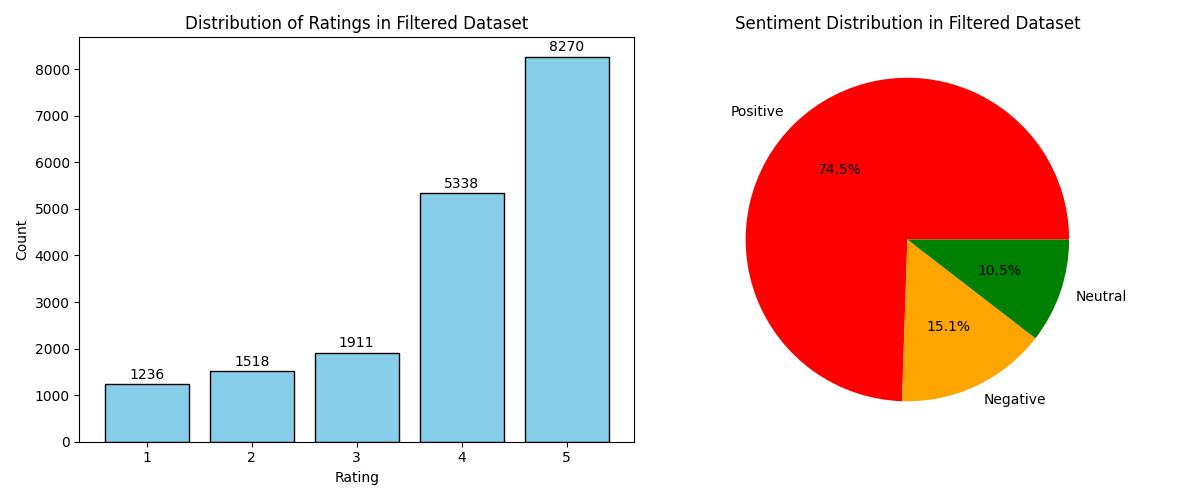
\includegraphics[width=\textwidth]{images/label_distribution.png}
            \caption{Label distribution}
        \end{figure}
        The dataset is quite unbalanced, with a vast majority of positive reviews (4-5 stars). 

        The reviews were then split into:
        \begin{itemize}
            \item training set: $72.3\%$
            \item validation set: $12.7\%$
            \item test set: $15\%$
        \end{itemize}

        Based on the used model, the reviews were converted to tokens either using The
        RoBERTa tokenizer, either using the NLTK tokenizer, which was used to create the
        vocabulary for the RNN model. Both tokenized datasets were then padded to a maximum 
        length of 256 tokens.

    \subsection{Models}
    \label{subsec:models}
        \subsubsection{LSTM-RNN}
        \label{subsubsec:lstm}
            The first model implemented is a Long Short-Term Memory (LSTM) Recurrent
            Neural Network (RNN) implemented in Torch, made of:
            \begin{itemize}
                \item an embedding layer, which converts the input tokens to a dense vector representation;
                \item a LSTM layer, which processes the sequence of embeddings and captures the sequence temporal dependencies;
                \item a fully connected layer, which maps the output of the LSTM to the final output classes.
                \item a softmax activation function
            \end{itemize}

            \begin{figure}[H]
                \centering
                \begin{tikzpicture}[
                    node distance=0.8cm and 0.5cm,
                    every node/.style={align=center, font=\scriptsize},
                    layer/.style={draw, rounded corners, minimum height=0.9cm, minimum width=1.8cm, text centered},
                    input/.style={layer, fill=blue!20},
                    embed/.style={layer, fill=orange!30},
                    lstm/.style={layer, fill=purple!25},
                    dense/.style={layer, fill=green!25},
                    softmax/.style={layer, fill=red!25},
                    output/.style={layer, fill=gray!20}
                ]

                    % Nodes (horizontal layout)
                    \node (input) [input] {Input};
                    \node (embedding) [embed, right=of input] {Embedding};
                    \node (lstm) [lstm, right=of embedding] {LSTM + \\ Dropout};
                    \node (fc) [dense, right=of lstm] {Mean Pooling + \\ Dense Layer};
                    \node (sm) [softmax, right=of fc] {Softmax};
                    \node (out) [output, right=of sm] {Output \\ Class};

                    % Arrows
                    \draw[->, thick] (input) -- (embedding);
                    \draw[->, thick] (embedding) -- (lstm);
                    \draw[->, thick] (lstm) -- (fc);
                    \draw[->, thick] (fc) -- (sm);
                    \draw[->, thick] (sm) -- (out);

                \end{tikzpicture}
                \caption{LSTM-based sentiment classifier.}
            \end{figure}

            In particular, to evaluate the performance of the model, only the
            higher probability class is selected.
            The model is trained using the ADAM optimizer \citep{kingma2017adam},
            based on the cross-entropy loss function. Some form of dropout
            is applied to the LSTM layer to avoid overfitting.
            the model is trained for a maximum of 100 epochs, with early stopping
            kicking in almost always before the epochs upper limit, based on the 
            f1 score on the validation set.\\

            The tokenizer used in this model, as said before, is the NLTK tokenizer,
            with a vocabulary size of 10002, corresponding to the 10000 most
            frequent words in the training set, plus the \texttt{<PAD>} and \texttt{<OOV>} tokens,
            corresponding to the padding token and the out-of-vocabulary token.


        \subsubsection{RoBERTa Transformer}
        \label{subsubsec:roberta}
            The second model implemented is a \texttt{RoBERTaForSequenceClassification} transformer
            from the HuggingFace Transformers library, initialized at the \textit{roberta-base} 
            checkpoint. Furthermore, a classification MLP head is present, that takes information 
            from the first output of the RoBERTa transformer, which corresponds to the 
            \texttt{[CLS]} token, and maps it to the final output classes using softmax activation.

            \begin{figure}[H]
                \centering
                \begin{tikzpicture}[
                    node distance=0.8cm and 0.5cm,
                    every node/.style={align=center, font=\scriptsize},
                    layer/.style={draw, rounded corners, minimum height=0.9cm, minimum width=2.2cm, text centered},
                    input/.style={layer, fill=blue!20},
                    roberta/.style={layer, fill=orange!20},
                    mlp/.style={layer, fill=green!20},
                    softmax/.style={layer, fill=red!25},
                    output/.style={layer, fill=gray!20}
                ]

                    % Nodes (horizontal layout)
                    \node (input) [input] {Input};
                    \node (encoder) [roberta, right=of input] {RoBERTa\\(\texttt{roberta-base}) \\ + LoRA};
                    \node (mlp) [mlp, right=of encoder] {MLP Head\\(on [CLS])};
                    \node (sm) [softmax, right=of mlp] {Softmax};
                    \node (out) [output, right=of sm] {Output \\ Class};

                    % Arrows
                    \draw[->, thick] (input) -- (encoder);
                    \draw[->, thick] (encoder) -- (mlp);
                    \draw[->, thick] (mlp) -- (sm);
                    \draw[->, thick] (sm) -- (out);

                \end{tikzpicture}
                \caption{RoBERTa-based sentiment classifier.}
            \end{figure}

            The model, even though is pretrained, is fine-tuned on the datset using a rank-32 LoRA (Low-Rank Adaptation) PEFT
            with dropout. Like with the LSTM-RNN model the training has place using the cross-entropy loss function, 
            with the optimization performed using the ADAMW optimizer \citep{loshchilov2019decoupledweightdecayregularization}
            It should be noted that the model is trained using fp16 mixed precision, allowing
            to speed up the training and reducing the memory usage, allowing the
            training of the model on a single GPU with 6GB of memory.\\

            Furthermore, a Learning Rate Warmup \citep{kalra2024warmuplearningrateunderlying} of 10\% of the training steps
            is applied.
            The tokenizer used in this model is the \textit{roberta-base} tokenizer.